% Original source: Zhou, physical PDF pp. 80--84 (printed pp. 64--68).
% Figures: Figure 4.1 is recreated with native TikZ.
% Uncertainty log: none.

% ZHOU-SOURCE-PAGE: 80 PRINTED: 64

other points within a clockwise semicircle. Figure 4.1 clearly demonstrates this
conclusion. If starting at point $i$ and proceeding clockwise along the circle, we
sequentially encounter points $i+1$, $i+2$, $\ldots$, $N$, $1$, $\ldots$, $i-1$ within
half a circle, the clockwise arc between $i-1$ and $i$ must be no less than half a
circle. If we start at any other point, in order to reach all other points clockwise,
the clockwise arc between $i-1$ and $i$ are always included. So we cannot reach all
points within a clockwise semicircle starting from any other points. Hence, all these
events are mutually exclusive and we have

\[
P\left(\bigcup_{i=1}^{N}E_i\right)
=\sum_{i=1}^{N}P(E_i)
\Rightarrow
P\left(\bigcup_{i=1}^{N}E_i\right)
=N\cdot\frac{1}{2^{N-1}}
=\frac{N}{2^{N-1}}.
\]

The same argument can be extended to any arcs that have a length less than half a
circle. If the ratio of the arc length to the circumference of the circle is $x$
($x\leq1/2$), then the probability of all $N$ points fitting into the arc is
$N\cdot x^{N-1}$.
\end{solution}

\begin{figure}[ht]
\centering
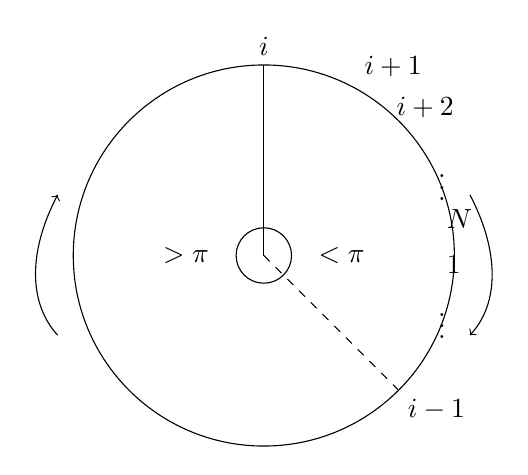
\begin{tikzpicture}[scale=1.1]
  \coordinate (I) at (0,2.2);
  \coordinate (ImOne) at (1.55,-1.55);
  \draw (0,0) circle (2.2);
  \draw (I) -- (0,0);
  \draw[dashed] (0,0) -- (ImOne);
  \draw (0,0) circle (0.32);
  \node[above] at (I) {$i$};
  \node[above right] at (1.05,1.95) {$i+1$};
  \node[above right] at (1.42,1.48) {$i+2$};
  \node[right] at (1.90,0.88) {$\vdots$};
  \node[right] at (2.00,0.42) {$N$};
  \node[right] at (2.00,-0.10) {$1$};
  \node[right] at (1.90,-0.72) {$\vdots$};
  \node[below right] at (ImOne) {$i-1$};
  \node[left] at (-0.52,0) {$>\pi$};
  \node[right] at (0.52,0) {$<\pi$};
  \draw[->] (2.38,0.70) .. controls (2.72,0.05) and (2.72,-0.55) .. (2.38,-0.92);
  \draw[->] (-2.38,-0.92) .. controls (-2.72,-0.55) and (-2.72,0.05) .. (-2.38,0.70);
\end{tikzpicture}
\caption{$N$ points fall in a clockwise semicircle starting from $i$}
\label{fig:zhou-figure-4-1}
\end{figure}

\subsection{Combinatorial Analysis}

Many problems in probability theory can be solved by simply counting the number of
different ways that a certain event can occur. The mathematic theory of counting is
often referred to as combinatorial analysis (or combinatorics). In this section, we will
cover the basics of combinatorial analysis.

\begin{concept}{Combinatorial principles}
\noindent\emph{Basic principle of counting:} Let $S$ be a set of length-$k$ sequences.
If there are

% ZHOU-SOURCE-PAGE: 81 PRINTED: 65
\begin{itemize}
\item $n_1$ possible first entries,
\item $n_2$ possible second entries for each first entry,
\item $n_3$ possible third entries for each combination of first and second entries, etc.
\end{itemize}

Then there are a total of $n_1\cdot n_2\cdots n_k$ possible outcomes.

\noindent\emph{Permutation:} A rearrangement of objects into distinct sequence
(i.e., order matters).

\noindent\emph{Property:} There are
\[
\frac{n!}{n_1!n_2!\ldots n_r!}
\]
different permutations of $n$ objects, of which $n_1$ are alike, $n_2$ are alike,
$\ldots$, $n_r$ are alike.

\noindent\emph{Combination:} An unordered collection of objects (i.e., order
doesn't matter).

\noindent\emph{Property:} There are
\[
\binom{n}{r}=\frac{n!}{(n-r)!r!}
\]
different combinations of $n$ distinct objects taken $r$ at a time.

\noindent\emph{Binomial theorem:}
\[
(x+y)^n=\sum_{k=0}^{n}\binom{n}{k}x^k y^{n-k}.
\]

\noindent\emph{Inclusion-Exclusion Principle:}
\[
P(E_1\cup E_2)=P(E_1)+P(E_2)-P(E_1E_2)
\]
\[
P(E_1\cup E_2\cup E_3)
=P(E_1)+P(E_2)+P(E_3)-P(E_1E_2)-P(E_1E_3)-P(E_2E_3)+P(E_1E_2E_3)
\]
And more generally,
\[
\begin{aligned}
P(E_1\cup E_2\cup\ldots\cup E_N)
={}&\sum_{i=1}^{N}P(E_i)
-\sum_{i_1<i_2}P(E_{i_1}E_{i_2})
+\cdots+(-1)^{r+1}\sum_{i_1<i_2<\cdots<i_r}\\
&\qquad P(E_{i_1}E_{i_2}\cdots E_{i_r})+\cdots\\
&+(-1)^{N+1}P(E_1E_2\cdots E_N).
\end{aligned}
\]
Where
\[
\sum_{i_1<i_2<\cdots<i_r}P(E_{i_1}E_{i_2}\cdots E_{i_r})
\]
has $\binom{N}{r}$ terms.
\end{concept}

\subsubsection{Poker hands}

Poker is a card game in which each player gets a hand of 5 cards. There are 52 cards in
a deck. Each card has a value and belongs to a suit. There are 13 values,
\[
2,\ 3,\ 4,\ 5,\ 6,\ 7,\ 8,\ 9,\ 10,\
\underbrace{J}_{\text{jack}},\
\underbrace{Q}_{\text{queen}},\
\underbrace{K}_{\text{king}},\
\underbrace{A}_{\text{ace}},
\]
and four suits, $\spadesuit$, $\clubsuit$, $\heartsuit$, $\diamondsuit$.

% ZHOU-SOURCE-PAGE: 82 PRINTED: 66
\begin{problem}{What are the probabilities of getting hands with four-of-a-kind (four of the five cards with the same value)? Hands with a full house (three cards of one value and two cards of another value)? Hands with two pairs?}
\end{problem}
\begin{solution}
The number of different hands of a five-card draw is the number of 5-element subsets
of a 52-element set, so total number of hands
\[
=\binom{52}{5}=2,598,960.
\]

\noindent\emph{Hands with a four-of-a-kind:} First we can choose the value of the four
cards with the same value, there are 13 choices. The 5th card can be any of the rest 48
cards (12 choices for values and 4 choices for suits). So the number of hands with
four-of-a-kind is
\[
13\cdot48=624.
\]

\noindent\emph{Hands with a Full House:} In sequence we need to choose the value of the
triple, 13 choices; the suits of the triple, $\binom{4}{3}$ choices; the value of the
pair, 12 choices; and the suits of the pair, $\binom{4}{2}$ choices. So the number of
hands with full house is
\[
13\cdot\binom{4}{3}\cdot12\cdot\binom{4}{2}
=13\cdot4\cdot12\cdot6=3,744.
\]

\noindent\emph{Hands with Two Pairs:} In sequence we need to choose the values of the
two pairs, $\binom{13}{2}$ choices; the suits of the first pair, $\binom{4}{2}$ choices;
the suits of the second pair, $\binom{4}{2}$ choices; and the remaining card, 44
($52-4\cdot2$, since the last cards can not have the same value as either pair)
choices. So the number of hands with two pairs is
\[
\binom{13}{2}\cdot\binom{4}{2}\cdot\binom{4}{2}\cdot44
=78\cdot6\cdot6\cdot44=123,552.
\]

To calculate the probability of each, we only need to divide the number of hands of each
kind by the total possible number of hands.
\end{solution}

\begin{problem}{Hopping rabbit}
A rabbit sits at the bottom of a staircase with $n$ stairs. The rabbit can hop up only one
or two stairs at a time. How many different ways are there for the rabbit to ascend to the
top of the stairs?\footnotemark[5]

\footnotetext[5]{Hint: Consider an induction approach. Before the final hop to reach the
$n$-th stair, the rabbit can be at either the $(n-1)$th stair or the $(n-2)$th stair
assuming $n>2$.}
\end{problem}

% ZHOU-SOURCE-PAGE: 83 PRINTED: 67
\begin{solution}
Let's begin with the simplest cases and consider solving the problem for any number of
stairs using induction. For $n=1$, there is only one way and $f(1)=1$. For $n=2$, we can
have one 2-stair hop or two 1-stair hops. So $f(2)=2$. For any $n>2$, there are always two
possibilities for the last hop, either it's a 1-stair hop or a 2-stair hop. In the former
case, the rabbit is at $(n-1)$ before reaching $n$, and it has $f(n-1)$ ways to reach
$(n-1)$. In the latter case, the rabbit is at $(n-2)$ before reaching $n$, and it has
$f(n-2)$ ways to reach $(n-2)$. So we have
\[
f(n)=f(n-2)+f(n-1).
\]
Using this function we
can calculate $f(n)$ for $n=3$, $4$, $\ldots$\footnotemark[6]
\end{solution}

\footnotetext[6]{You may have recognized that the sequence is a sequence of Fibonacci
numbers.}

\begin{problem}{Screwy pirates 2}
Having peacefully divided the loot (in chapter 2), the pirate team goes on for more
looting and expands the group to 11 pirates. To protect their hard-won treasure, they
gather together to put all the loot in a safe. Still being a democratic bunch, they decide
that only a majority -- any majority -- of them ($\geq6$) together can open the safe. So
they ask a locksmith to put a certain number of locks on the safe. To access the treasure,
every lock needs to be opened. Each lock can have multiple keys, but each key only opens
one lock. The locksmith can give more than one key to each pirate.

What is the smallest number of locks needed? And how many keys must each pirate carry?
\footnotemark[7]
\end{problem}

\begin{solution}
This problem is a good example of the application of combinatorial analysis in information
sharing and cryptography. A general version of the problem was explained in a 1979 paper
\textquotedblleft How to Share a Secret\textquotedblright by Adi Shamir. Let's randomly select
5 pirates from the 11-member group; there must be a lock that none of them has the key to.
Yet any of the other 6 pirates must have the key to this lock since any 6 pirates can open
all locks. In other words, we must have a \textquotedblleft special\textquotedblright lock to
which none of the 5 selected pirates has a key and the other 6 pirates all have keys. Such
5-pirate groups are randomly selected. So for each combination of 5 pirates, there must be
such a \textquotedblleft special\textquotedblright lock. The minimum number of locks needed
is
\[
\binom{11}{5}=\frac{11!}{5!6!}=462
\]
locks. Each lock has 6 keys, which are given to a unique 6-member subgroup. So each pirate
must have
\[
\frac{462\cdot6}{11}=252
\]
keys. That's surely a lot of locks to put on a safe and a lot of keys for each pirate to
carry.
\end{solution}

\footnotetext[7]{Hint: every subgroup of 6 pirates should have the same key to a unique lock
that the other 5 pirates do not have.}

% ZHOU-SOURCE-PAGE: 84 PRINTED: 68
\begin{problem}{Chess tournament}
A chess tournament has $2^n$ players with skills $1>2>\cdots>2^n$. It is organized as a
knockout tournament, so that after each round only the winner proceeds to the next round.
Except for the final, opponents in each round are drawn at random. Let's also assume that
when two players meet in a game, the player with better skills always wins. What's the
probability that players 1 and 2 will meet in the final?\footnotemark[8]
\end{problem}

\begin{solution}
There are at least two approaches to solve the problem. The standard approach applies
multiplication rule based on conditional probability, while a counting approach is far more
efficient. (We will cover conditional probability in detail in the next section.)

Let's begin with the conditional probability approach, which is easier to grasp. Since there
are $2^n$ players, the tournament will have $n$ rounds (including the final). For round 1,
players $2,3,\ldots,2^n$ each have $\dfrac{1}{2^n-1}$ probability to be 1's rival, so the
probability that
\[
1\text{ and }2\text{ do not meet in round 1}
=\frac{2^n-2}{2^n-1}
=\frac{2\cdot(2^{n-1}-1)}{2^n-1}.
\]
Condition on that 1 and 2 do not meet in round 1, $2^{n-1}$ players proceed to the 2nd
round and the conditional probability that 1 and 2 will not meet in round 2 is
\[
\frac{2^{n-1}-2}{2^{n-1}-1}
=\frac{2\cdot(2^{n-2}-1)}{2^{n-1}-1}.
\]
We can repeat the same process until the $(n-1)$th round, in which there are
$2^2$ ($=2^n/2^{n-2}$) players left and the conditional probability that 1 and 2 will
not meet in round $(n-1)$ is
\[
\frac{2^2-2}{2^2-1}
=\frac{2\cdot(2^{2-1}-1)}{2^2-1}.
\]

Let $E_1$ be the event that 1 and 2 do not meet in round 1;

\[
E_2\text{ be the event that 1 and 2 do not meet in rounds 1 and 2;}
\]

\[
\ldots
\]

\[
E_{n-1}\text{ be the event that 1 and 2 do not meet in round 1,2,\ldots,n-1.}
\]

Apply the multiplication rule, we have
\[
\begin{aligned}
P(1\text{ and }2\text{ meet in the }n\text{th game})
={}&P(E_1)\cdot P(E_2\vert E_1)\cdot\cdots\\
&\cdot P(E_{n-1}\vert E_1,E_2,\ldots,E_{n-2})\\
={}&\frac{2\cdot(2^{n-1}-1)}{2^n-1}
\cdot\frac{2\cdot(2^{n-2}-1)}{2^{n-1}-1}\\
&\cdot\cdots\cdot\frac{2\cdot(2^{2-1}-1)}{2^2-1}\\
={}&\frac{2^{n-1}}{2^n-1}.
\end{aligned}
\]

\end{solution}

\footnotetext[8]{Hint: Consider separating the players to two $2^{n-1}$ subgroups. What
will happen if player 1 and 2 in the same group? Or not in the same group?}
